% !TEX root = diss.tex

\chapter{Introduction}

\section{Background}

Radicals are chemical species which tend to be highly reactive due to the presence of one or more unpaired electrons. Living systems depend on radical processes as part of normal metabolism\cite{Halliwell2015} but biomaterials, such as proteins, are susceptible to radical induced damage. Radical induced oxidation of biomaterials has been implicated in a number of degenerative disease states, including cancer, Alzheimer's Disease, Parkinson's Disease, and multiple sclerosis.\cite{Barnham2004, Valko2007, Hwang2013, Halliwell2007}

In biological systems, radicals are derived from many sources. Exogenous sources include solar radiation and air pollutants, while endogenous sources include \emph{in vivo} transition metal-ion redox processes, such as the electron transport chain involved in cellular respiration.\cite{Turrens2003} Some redox centres in the electron transport chain may uncontrollably transfer an electron to molecular oxygen, forming the superoxide anion (\ch{O2^{.-}}). Superoxide is not a strong oxidant on its own, however, it may disproportionate, either spontaneously or catalytically through metalloenzymes such as superoxide dismutase, leading to more reactive oxygen-centred radicals. In fact, most oxygen-centred radicals derive from reactions of \ch{O2} with redox-active metals.\cite{Halliwell2015}

Oxygen-centred radicals, known as reactive oxygen species (ROSs) in biology, are particularly important and common due to the nature of the aerobic respiration. The ROSs which are of primary concern are the highly reactive hydroxyl radical (\ch{HO^.}), alkoxyl radicals (\ch{RO^.}), superoxide (\ch{HOO^.}/\ch{O2^{.-}}), and peroxyl radicals (\ch{ROO^.}).\cite{Halliwell2015} Radical induced oxidation, or oxidative stress, occurs when an ROS initiates a radical chain reaction through hydrogen atom transfer (HAT), electron transfer, or addition reactions, leading to rapid propagation. HAT is the most relevant reaction, and thus is the focus of my work.

This work is primarily concerned with developing an understanding of the fundamental chemistry involved in protein oxidation. Proteins are the most abundant biomaterial in most biological systems,\cite{Davies2005} thus understanding their degradation is essential to understanding degenerative disease. The oxidation of protein by ROSs occurs through a radical chain mechanism which has been studied in detail.\cite{Berlett1997, Davies2016} As proteins contain as many as 20 common amino acid side chains, as well as the common peptide backbone, there are a large number of possible reactions.  Some of the reactions involved in protein oxidation are shown in~\ref{fig:proteinoxidation}.

\begin{scheme}[h!]
  \centering
  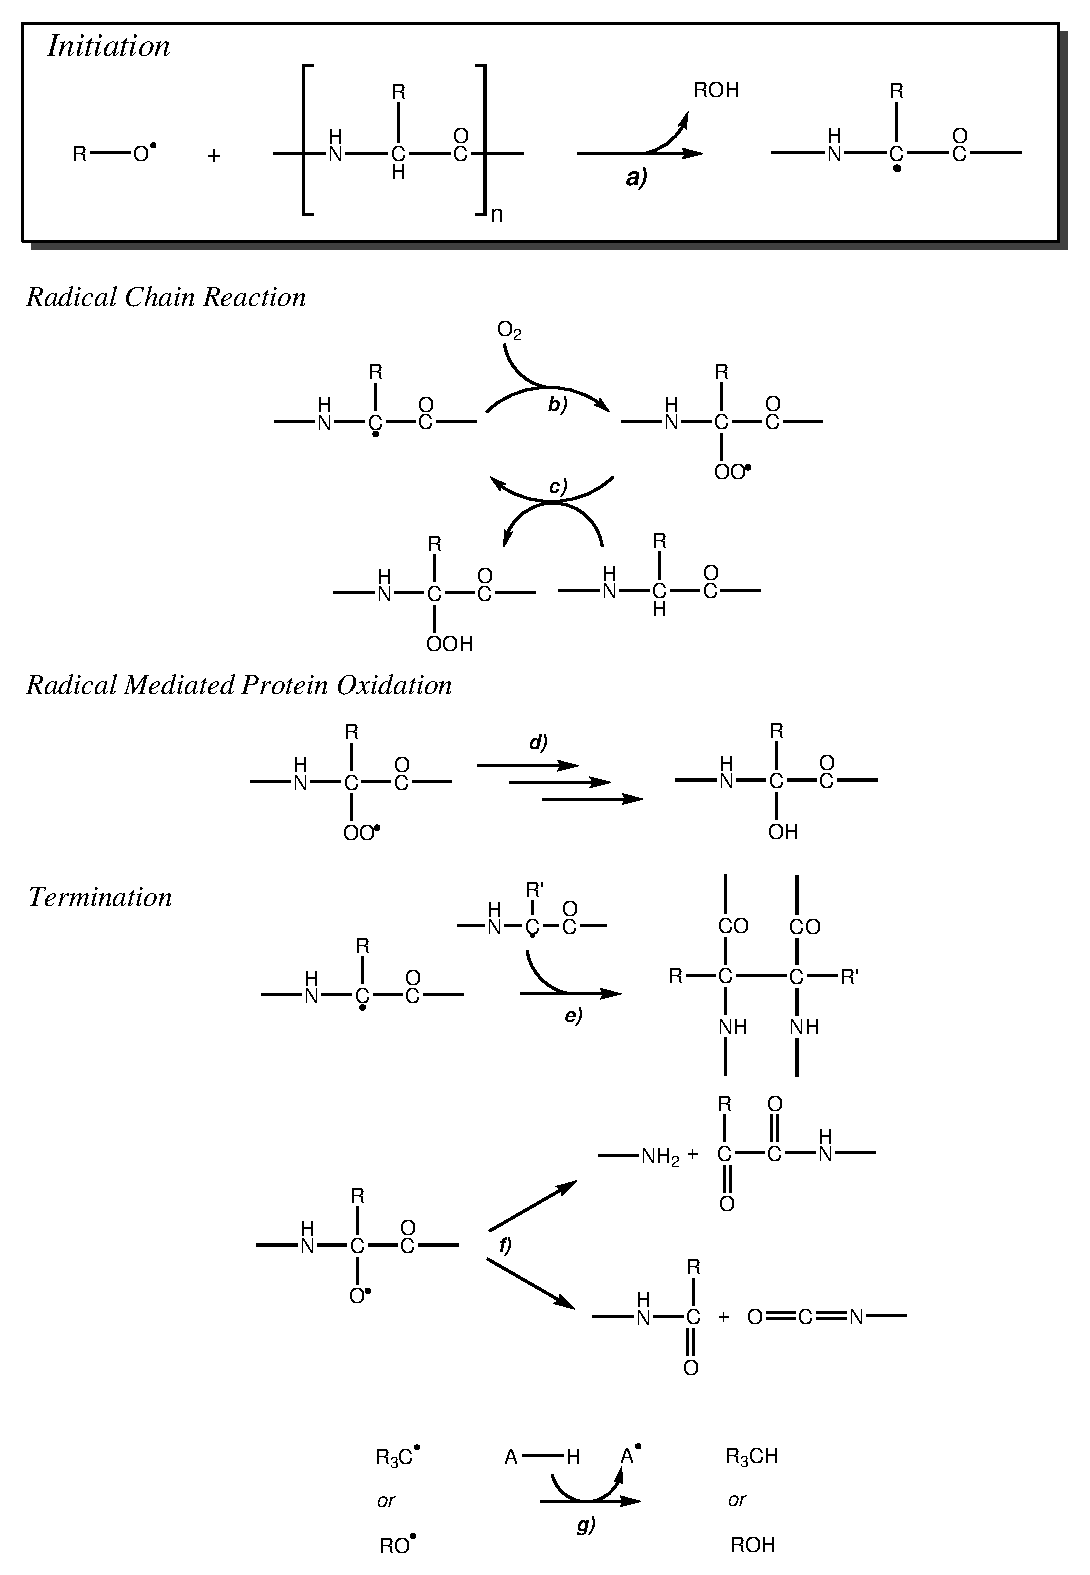
\includegraphics[height=12cm]{figures/proteinoxidation-2.eps}
\caption[Common reactions involved in the protein oxidation.]{Common reaction involved in the protein oxidation. The reactions are as follows: \textbf{a} initiation of radical chain through abstraction by an oxygen centred radical to generate an $\alpha$-carbon radical, \textbf{b)} radical addition of molecular oxygen, \textbf{c)} propagation of the radical chain reaction generating another $\alpha$-carbon radical and an peroxide. \textbf{d)} Radical mediated protein oxidation proceeds through multiple steps involving oxygen centred radicals and molecular oxygen result in the generation of a hydrogen-amide. Termination of the radical chain reaction can occur in several ways, including: \textbf{e)} possible cross-linking mechanism of two carbon-centred radicals, \textbf{f)} possible fragmentation pathways of an oxygen-centred radical intermediate, or \textbf{g)} HAT with an antioxidant.}
\label{fig:proteinoxidation}
\end{scheme}

Initial abstraction (Reaction \textbf{a}) often occurs at the $\alpha$-carbon position (\ch{$\alpha$-CH}), forming a carbon-centred radical (\ch{$\alpha$-C^.}) which is partially delocalised in the $\pi$-system of the neighbouring amide and carbonyl groups. Many studies have indicated that the stability of \ch{$\alpha$-C^.} is determined by stereo-electronic considerations related to the planarity of the amide group. Hence, steric bulk of the side chains, as well as local protein structure (helix, sheet, etc.) can constrain radical geometries. For example, the most stable $\alpha$-carbon radicals occur at glycine residues in antiparallel $\beta$-sheets, as other bulkier residues and secondary structures lead to loss of captodative stabilisation.\cite{Rauk2000} Amino acid side-chains are also susceptible to oxidation. Those side-chains containing sulphur,\cite{Stadtman2004} as well as tyrosine (which has a fairly weak phenolic O-H bond of about 89 \kcalmol),\cite{Mulder2005} are particularly susceptible to oxidation.

Propagation of the radical chain reaction occurs through various processes. In the presence of molecular oxygen, rapid addition occurs at to the newly formed \ch{$\alpha$-C^.} (Reaction \textbf{b}), generating a peroxyl radical, which can carry forward through further HAT reactions (Reaction \textbf{c}).\cite{Stadtman2003} The mechanism involved in the radical mediated oxidation of proteins has been studied experimentally using techniques involving ionising radiation.\cite{Garrison1962,Garrison1987} The course of this process is complexly dependent on the availability of either singlet oxygen (\ch{^1O2}), or superoxide (\ch{O2^{.-}}) (or the protonated form, peroxyl radical (\ch{^.OOH})). A detailed analysis of this process is outside the scope of thesis, but ultimately, these reactions lead to the generation of a hydroxyl-amide (Reaction \textbf{d}).

The radical chain reaction can be terminated through several mechanisms, including protein-protein cross-linking (Reaction \textbf{e}), protein fragmentation (Reaction \textbf{f}), or reactions with antioxidants (\ch{A-H}, Reaction \textbf{g}). The sum total of all these processes contribute to the accumulation of oxidised proteins which is associated with many degenerative diseases.\cite{Halliwell2006} HAT reactions which are important steps in the initiation, propagation, and termination reactions of protein oxidation are investigated herein.

\section{Studying HAT reactions}

Developing an understanding of protein and other biomolecular oxidation requires an understanding of the deceptively simple HAT reactions involved. Formal HAT reactions are a fundamental radical chemical transformation which have been studied for over a century.\cite{Kochi1973, Parsons2000} From an experimental perspective, HAT reactions which involve oxygen-centred radicals, and non-radical organic substrates, are reasonably well characterised: the effects of bulk solvent are well understood.\cite{Litwinienko2007} However, the main challenge faced by many experiments is elucidating the mechanistic details of a reaction. This is a problem that can be examined by quantum chemistry, which is the approach that I shall take. Background on the theory used in this thesis is given in Chapter~\ref{ch:theory}.

In order to investigate HAT reactions, we need to consider the mechanism in detail. For a simple HAT reaction, there exists several possible mechanisms by which this transformation can occur. The two most common concerted mechanisms are direct HAT\footnotemark~ and proton-coupled electron transfer (PCET). At the basic level, direct HAT involves the transfer of an electron and proton through the same set of acceptor/donor orbitals, while PCET involves the transfer of an electron and proton through different sets of orbitals. In practise, this distinction is poorly described, and this topic is still in active discussion in the literature.\cite{Cukier1998, Mayer2002, Stubbe2003, Mayer2004, DiLabio2007, Huynh2007, HammesSchiffer2008, Mayer2010, Weinberg2012, HammesSchiffer2015, MunozRugeles2017}

\footnotetext{Not to be confused with the net reaction of formal hydrogen atom transfer. The abbreviation HAT will be used interchangeably, although the distinction should be clear from context.}

The quintessential example when comparing direct HAT to PCET comes from the work of Mayer et al.,\cite{Mayer2002} which describes the self-exchange reactions of benzyl-toluene and phenoxyl-phenol, shown in~\ref{fig:self1}. In this work, the transition state (TS) structures were obtained through theoretical studies. These complexes are oriented so that the aromatic rings are trans relative to one another. In this geometry, the benzyl-toluene pair undergoes direct HAT, with the $2p-\pi$ orbital of the benzylic carbon radical oriented at the benzylic hydrogen on toluene, with little delocalisation of the radical into the $\pi$-system. This is an example of direct HAT, as the orbital containing the radical overlaps with the X-H $\sigma^*$ anti-bonding orbital, and thus the electron and proton are transferred through the same set of orbitals. Another indication of direct HAT is that the singly-occupied molecular orbital (SOMO) is of $\sigma$-symmetry.

\begin{scheme}[htb]
\vspace{1cm}
\begin{overpic}[width=0.75\textwidth]{figures/PhCH3-PhCH2.eps}
  \put(-10,25) {\large\textbf{A.}}
\end{overpic}
\begin{overpic}[width=0.75\textwidth]{figures/PhOH-PhO.eps}
  \put(-10,15) {\large\textbf{B.}}
\end{overpic}
\caption{Self-exchange reactions of the \textbf{A.} benzyl-toluene couple through direct HAT \textbf{B.} phenoxyl-phenol couple through PCET.}
\label{fig:self1}
\end{scheme}

For the phenoxyl-phenol pair, a fairly strongly hydrogen bonded pre-reaction complex is first formed with a binding enthalpy $\Delta H$ of -8.1 \kcalmol. As a result of this strong interaction, the TS structure is such that the phenoxyl radical occupies a $2p$ orbital, and therefore, cannot overlap with the H-O $\sigma^*$ anti-bonding orbital in order to undergo direct HAT.\@ However, this does allow the of the radical overlap with the $2p$ lone pair of the phenol moiety and the aromatic $\pi$ systems. Hence, the TS complex SOMO is of $\pi$-symmetry and highly delocalised, thus HAT occurs through a PCET mechanism. The reaction has an enthalpic barrier height $\Delta H^{\ddagger}$ of 5.0 \kcalmol relative to the hydrogen bonded complex, so that the barrier is 3.1 \kcalmol below the separated reactants.

The work by \citet{Mayer2002} suggests that hydrogen bonding is a necessary, but not sufficient condition for PCET to occur. This then implies that PCET is not possible between molecules which do not possess hydrogen bonding moieties, such as carbon atoms. Work by other authors has shown this to be untrue.\cite{Hatcher2007, DiLabio2007} In particular, \citet{DiLabio2007} demonstrated that this neglected the important contributions of $\pi-\pi$ interactions and lone pair-$\pi$ interactions. Additional calculations revealed the existence of a TS structure for the benzyl-toluene couple which is 3.7 \kcalmol lower in energy than previously reported. This structure orients the aromatic rings $34^\circ$ relative to one another, allowing for optimal $\pi-\pi$ overlap.

Analysis of the TS highest-occupied molecular orbital (HOMO) reveals bonding character between the two $\pi$-system, while the SOMO shows anti-bonding character between the $\pi$-systems, as well as and both C-H bonds. Thus, there exists a net partial bonding interaction between the two $\pi$-systems, opening up an additional electronic channel for PCET to occur. DiLabio and Johnson also suggest that the phenol-phenoxyl couple likely prefers a $\pi$-stacked TS structure, and compare this to a structural analogue, a naturally occurring tyrosyl-tyrosine couple, which also proceeds through a PCET mechanism. Additional work by \citet{MunozRugeles2017} confirmed the existence of a $\pi$-stacked TS structure for the phenol-phenoxyl couple. They used an approach which utilises natural population analysis along the intrinsic reaction coordinate, and demonstrated that both the benzyl-toluene couple and phenoxyl-phenol couple favour a $\pi$-stacked TS structure and undergo HAT through a PCET mechanism. Interestingly, they also showed that reaction barrier heights for the PCET mechanism are systematically lower than those for related direct HAT mechanism.

Bearing in mind there is not an obvious way to explore the differences in mechanism experimentally, computational examination of formal HAT reactions enables analysis of the mechanism of these reactions. Through careful investigation, a general distinction between a direct HAT mechanism and PCET mechanism can be achieved. In doing so, important insight is gained from understanding the electronic behaviour of these reactions. In this vein, the investigation of the physico-chemical nature of HAT reactions shall be the central theme of this thesis.

Consider for a moment the potential energy surface (PES) for an arbitrary chemical reaction, which is a complex hypersurface that depends on many variables. Theoretical methods can be used to generate a full PES, however, this quickly becomes computationally infeasible as the number of atoms in a system increases. Typically this problem can be simplified by examining only the relevant degrees of freedom. Often, the two most important coordinates can be isolated, giving a 3-dimensional PES.\@ Furthermore, in chemistry we often simplify this problem to 2-dimensions using the so-called intrinsic reaction coordinate, which is the lowest energy cross section of a higher dimension PES.\@ This yields a reaction coordinate diagram, as is illustrated below in~\ref{fig:pes}.

\begin{figure}[htb]
  \centering
  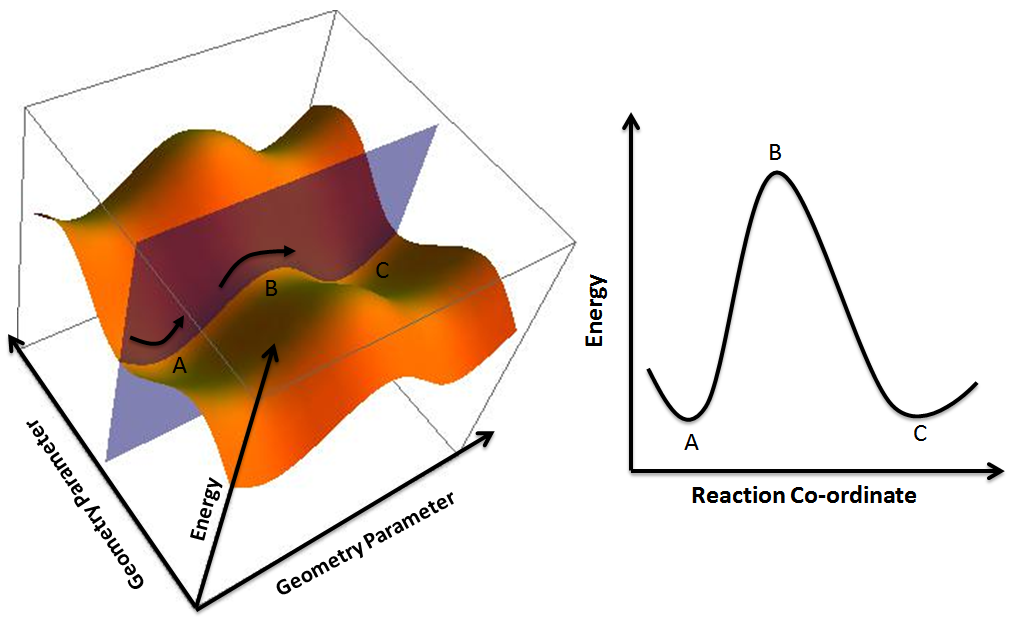
\includegraphics[width=0.9\textwidth]{figures/pes}
  \caption[A typical reaction coordinate diagram.]{A typical reaction coordinate diagram. Stationary states A, B, and C, correspond to the pre-reaction, transition state, and post-reaction complexes, respectively.}
\label{fig:pes}
\end{figure}

In a typical reaction coordinate diagram, the reactants begin to interact and form a pre-reaction complex (A). Given sufficient energy, the reaction will proceed over the top of the energy barrier through a transition state (TS) complex (B). After the chemical transformation is completed, a post-reaction complex (C) is formed until the products are able to separate. This is a somewhat na\"{i}ve description, as it only broadly describes a chemical transformation. In particular, the roles of substrate-radical and substrate-radical-medium interactions along the reaction coordinate are neglected. This is in fact a key point, as a thorough understanding of these interactions continues to be a hole in the literature.

Consequently, recent work from our group, in collaboration with our experimental colleagues at the University of Rome Tor Vergata, has focused on the importance of substrate-radical interactions in determining the kinetics of HAT reactions. Specifically, it has been shown that the three-dimensional structures of oxygen-centred radicals, as well as the organic substrates, impacts the nature of the interactions involved in HAT reaction pathways.\cite{Salamone2015Rev} In our work, we utilise primarily the benzyloxyl (\bno) and cumyloxyl (\cumo) radicals, which serve as a convenient proxy to biological oxygen-centred radicals. Reaction involving \bno and \cumo can be monitored using highly resolved laser flash photolysis (LFP) techniques. A combination of theoretical and experimental techniques have been used to examine reactions involving \bno and \cumo with a variety of organic substrates. A detailed discussion of these results shall be reserved for following chapters, however, a great deal of insight has been gained into the role of structure in both the radicals and substrates, and resulting intermolecular interactions.

With respect to the work in this thesis, in Chapter~\ref{ch:arrhenius} we shall consider the importance of the left-hand side of~\ref{fig:pes} by examining how the pre-reaction complex effects HAT reactions. There has been no detailed investigation of the importance of pre-reaction complex formation for HAT reaction. Oxygen-centred radicals can hydrogen bond with substrates as both acceptors and donors.\cite{Johnson2009a} These hydrogen bonding interactions, in addition to the other non-covalent interactions between the radical and substrate, lead to the formation of a pre-reaction complex. Accordingly, the formation of a pre-reaction complex is a fundamental step in protein oxidation.

The specific aim of this chapter is to investigate the effects of non-covalent binding in the pre-reaction complex with respect to the well known, but phenomenological Arrhenius equation. As of yet, there is no framework which relates the non-covalently bound pre-reaction complex to kinetic results. We ask the simple question: does there exists a direct correlation between the Arrhenius pre-factor and the non-covalent binding energy? To address this question, we examine the non-covalent binding in the pre-reaction complex in a series of related HAT reactions.

Arrhenius parameters for the systems of interest in this work were previously tabulated,\cite{DiLabio2005} and consist of thermoneutral or nearly thermoneutral reactions involving the creation and destruction of oxygen-centred radicals. These reactions are related to the phenol-phenoxyl self-exchange reaction, where a relatively strong pre-reaction complex is expected.

Then in Chapter~\ref{ch:bde}, we shall consider the right-hand side of~\ref{fig:pes}, where the effects of bond strengths on HAT rate constants are examined. Bond strengths are indicated by bond dissociation enthalpies (BDEs), and are central to the understanding of reactions with respect to thermodynamics. In addition to this, there exists a tremendous amount of literature in which BDEs are linked to chemical reactivity, especially for HAT reactions.\cite{Kochi1973, Tedder1982, Wijtmans2003, Pratt2004, Mayer2004} There exists a linear free energy relationship (LFER) called the Bell-Evans-Polanyi (BEP) Principle,\cite{Bell1936,Evans1938} which states that the difference in activation energy ($E_a$) for two related reactions, is proportional to the differences in reaction enthalpy ($\Delta H$):

\begin{equation}
  E_a = E_0 + \alpha \Delta H
  \label{eq:bep}
\end{equation}

\noindent where $E_0$ is the activation energy of a reference reaction, and $\alpha$, a constant which characterises the position of the TS along the reaction coordinate. This relationship can be more generally used to compare larger families of reactions. Despite the wide spread use of the BEP Principle, the applicability of this relationship is not well described.

I probe this applicability, with the aim to determine how generally the BEP principle can be applied. This is achieved by relating accurate, theoretically determined C-H bond strengths of species which undergo abstraction at these positions to the experimentally determined HAT rate constants. HAT reaction rate constants depend on many factors, however, by using measured rate constants from specific conditions (LFP with \cumo~at 298K), the difference in reactivity depend mainly on the differences in chemical properties of the substrates of interest. Therefore, we hypothesise that there should exist two BEP relationships for C-H bonds: one in which the incipient radical is delocalised into a $\pi$-system (benzylic-allylic), and the remaining alkyl radicals which are largely localised.

Finally, recent experimental results show that non-redox active metal cations, which are found ubiquitously in biological systems, have an inhibitory effect on HAT reactions involving oxygen-centred radicals. This has been demonstrated experimentally for substrates which undergo abstraction from sites adjacent to heteroatoms (e.g.\ amines, amides, and ethers). Under various stoichiometric ratios, these metal cations have effects ranging from full inhibition to partial deactivation of HAT reactivity.\cite{Salamone2013, Salamone2015metals, Salamone2016} This effect has been attributed partially to the effects of hyperconjugative overlap. Take for example tetrahydrofuran (THF), shown in~\ref{fig:THF}. Normally, there exists C-H bond weakening hyperconjugative overlap of electron density from one of the oxygen lone-pairs and the adjacent C-H $\sigma^*$ anti-bonding orbitals. The interaction of a metal cation with the oxygen lone-pairs removes electron density from this interaction, thus increasing the C-H bond strength. As a results, the reactivity of this bond is decreased, as observed from the experimentally measured 3.2-fold decrease in the rate constant for HAT with \cumo~in acetonitrile from 6.65 \E{7} \Ms to 7.0 \E{7} \Ms in the presence of 1.0 M \ch{Mg(ClO4)2}.\cite{Salamone2013}

\begin{scheme}[htb]
  \centering
  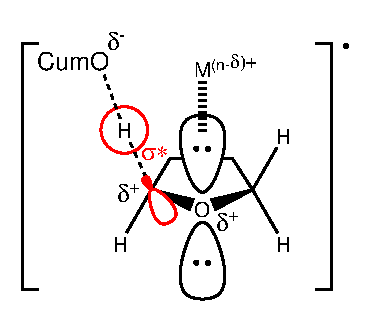
\includegraphics[width=0.65\textwidth]{figures/THF}
  \caption[Hyperconjugative overlap in tetrahydrofuran and the effect of non-redox active metal cations.]
  {Hyperconjugative overlap in tetrahydrofuran and the effect of non-redox active metal cations. The metal cation accepts electron density from the heteroatom lone pair, reducing overlap with the C-H $\sigma^*$ anti-bonding orbital and increasing the C-H bond strength.}
\label{fig:THF}
\end{scheme}

The nature of the interactions between non-redox active metal cations and organic substrates is poorly understood. The primary goal of this thesis is to understand the fundamental physico-chemical properties which lead to the experimentally observed trends in reactivity. This problem is explored in Chapter~\ref{ch:hat}. The experimentally observed effects have led us to hypothesise that the presence of non-redox active metal cations has a chemoprotective effect against the radical induced oxidation of biomaterials such as proteins.

In using theory to study HAT reactions, I hope to contribute to a better understanding of the fundamental properties which govern these reactions, and thus develop insights into the many important processes in which HAT takes place.
